%======================================================================
% CAPITULO 6: CHAT DE SANDRA AI
%======================================================================

\chapter{Chat de Sandra AI}
\label{ch:chat}

\sandraai{} no solo es un asistente de comandos, sino una interfaz conversacional completa que permite interactuar con el ecosistema SDC de forma natural e intuitiva. Este capitulo describe la interfaz de chat y sus capacidades avanzadas.

\section{Interfaz de Conversacion}
\label{sec:interfaz-chat}

El chat de Sandra AI proporciona un espacio de dialogo continuo donde los usuarios pueden realizar consultas, ejecutar comandos y recibir asistencia contextual.

\begin{figure}[H]
\centering
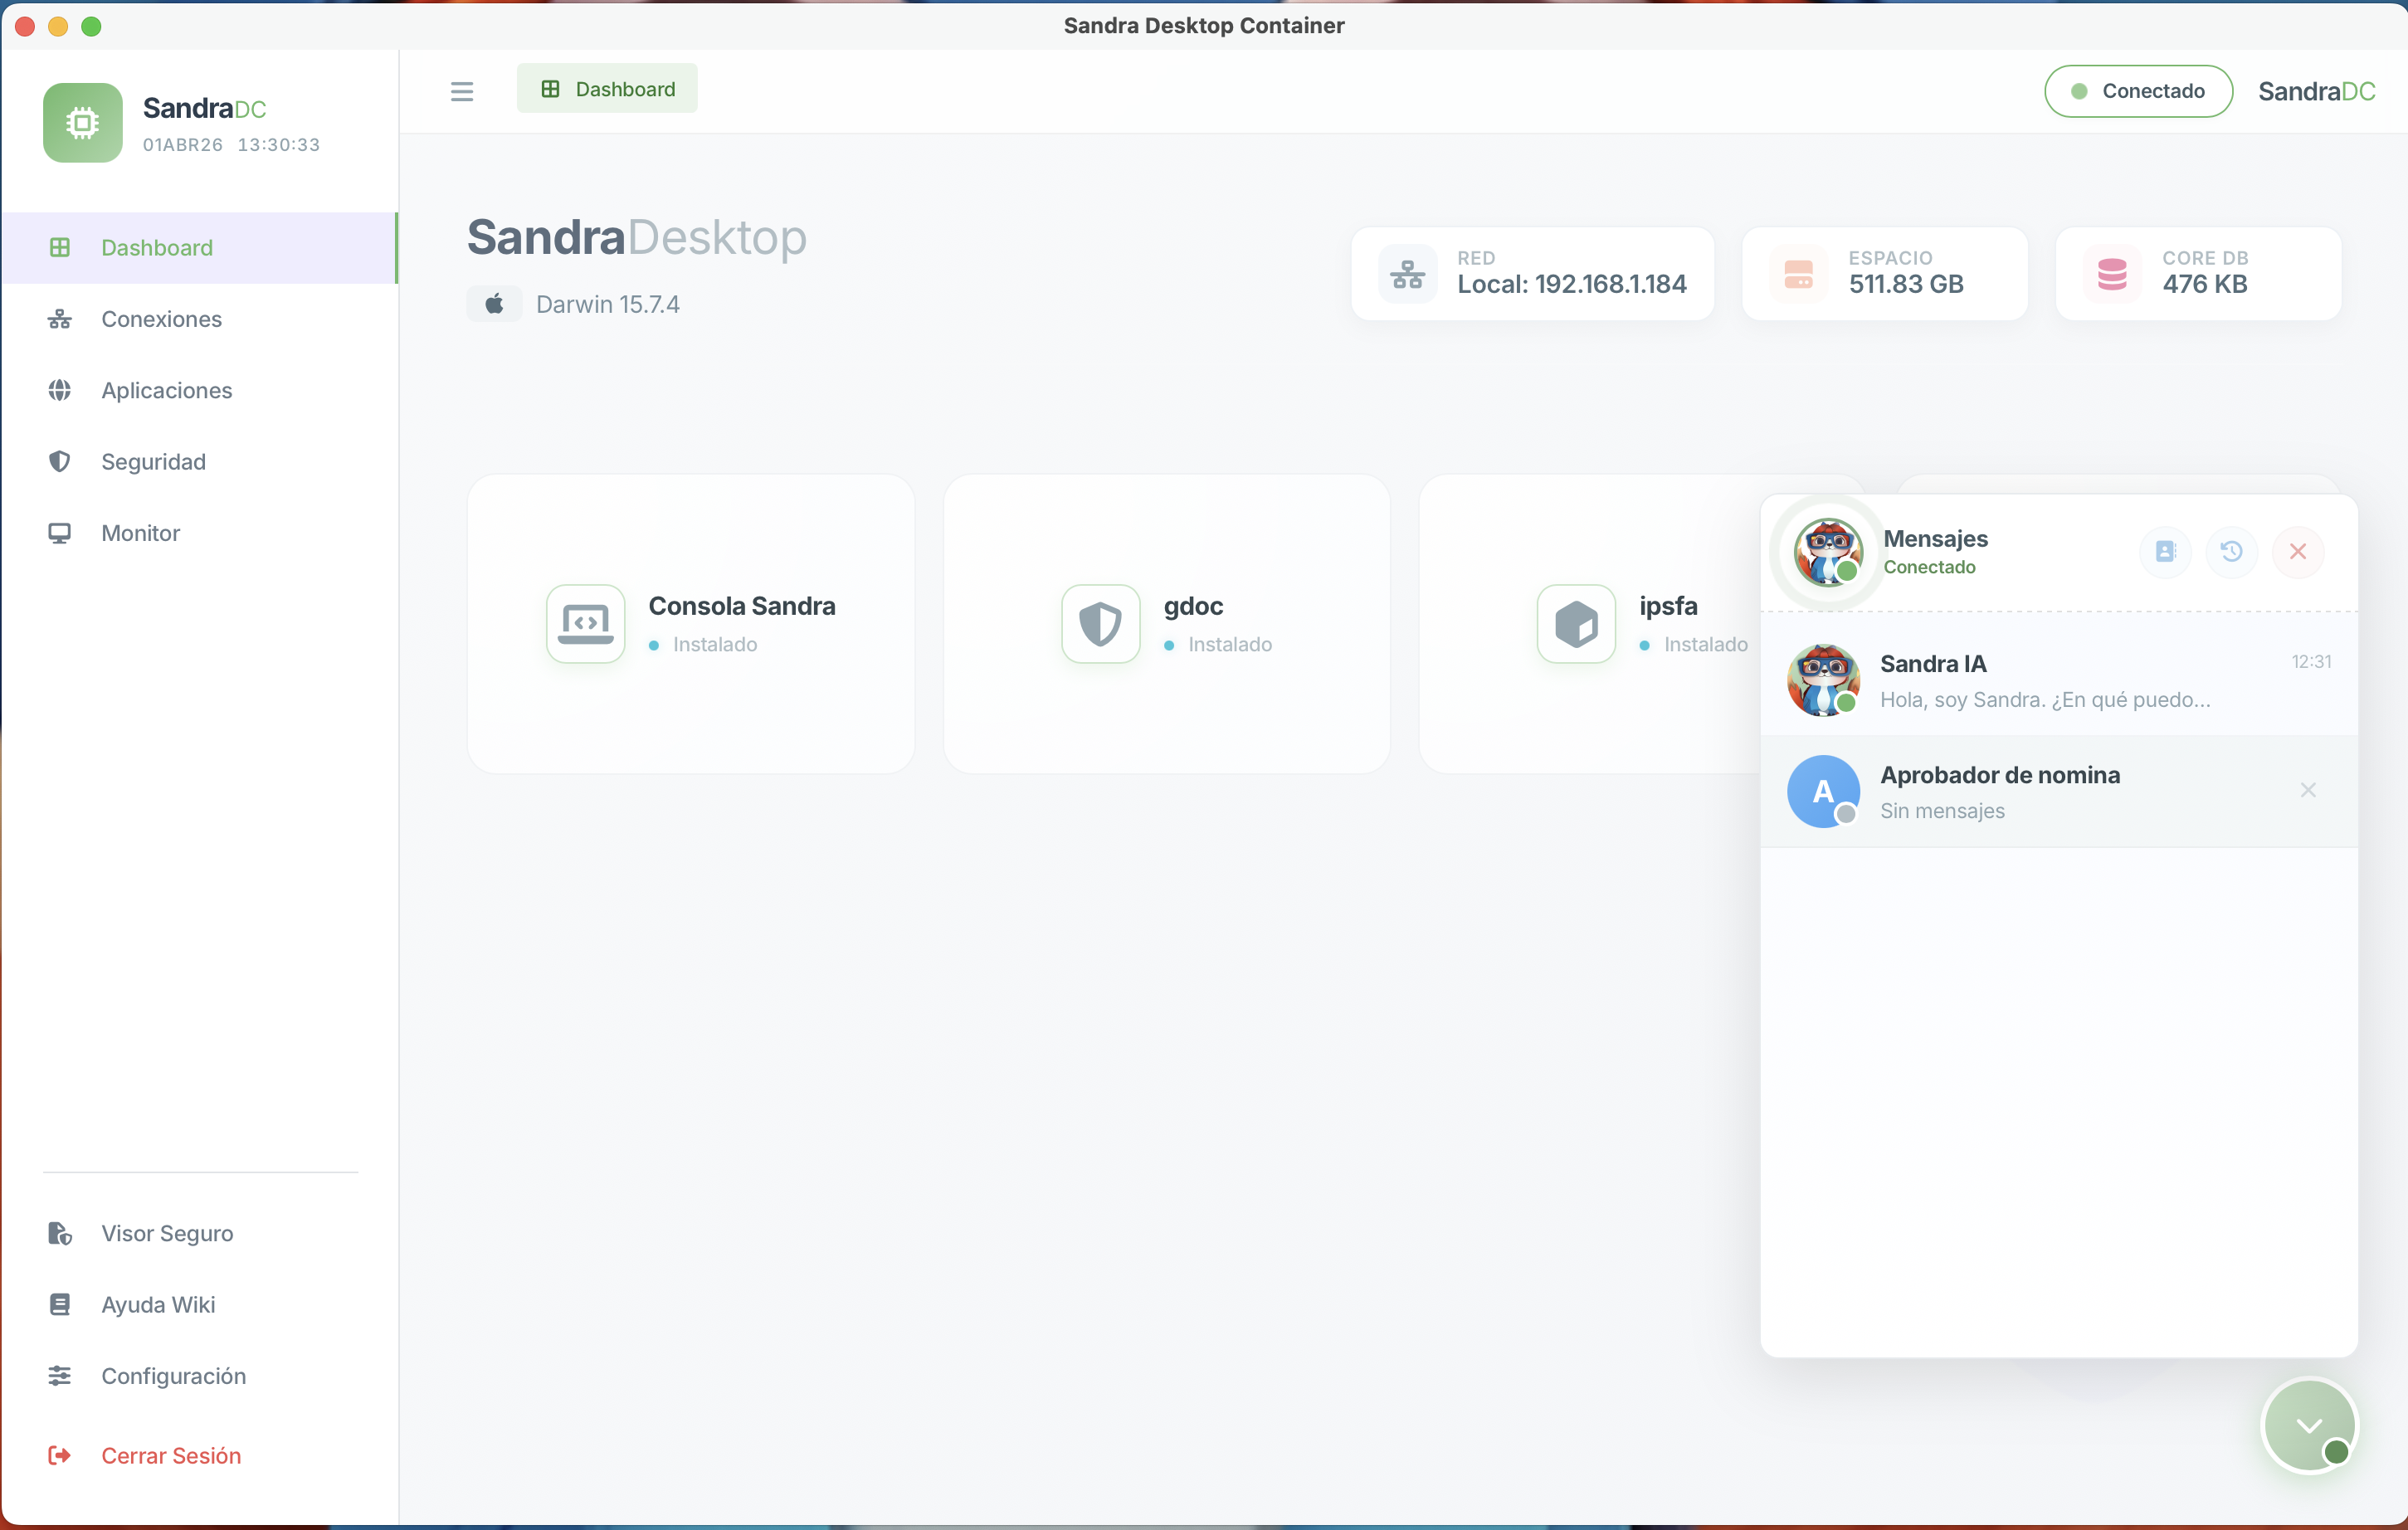
\includegraphics[width=0.95\textwidth]{anexos/22 chat.principal.png}
\caption{Interfaz de chat de Sandra AI}
\label{fig:chat}
\end{figure}

\subsection{Componentes de la Interfaz}

La interfaz de chat consta de los siguientes elementos:

\begin{itemize}[leftmargin=*]
    \item \textbf{Area de Mensajes}: Historial completo de la conversacion
    \item \textbf{Campo de Entrada}: Donde el usuario escribe sus consultas
    \item \textbf{Sugerencias Contextuales}: Comandos rapidos basados en el contexto actual
    \item \textbf{Indicador de Estado}: Muestra cuando Sandra esta procesando una respuesta
    \item \textbf{Botones de Accion}: Accesos directos a funciones frecuentes
\end{itemize}

\subsection{Historial de Conversaciones}

Sandra AI mantiene un historial persistente de conversaciones que incluye:

\begin{itemize}[leftmargin=*]
    \item \textbf{Contexto de Sesion}: Recuerda el tema de la conversacion actual
    \item \textbf{Referencias Cruzadas}: Puede referirse a elementos mencionados anteriormente
    \item \textbf{Aprendizaje Adaptativo}: Mejora las respuestas basandose en interacciones previas
    \item \textbf{Busqueda en Historial}: Permite recuperar informacion de conversaciones pasadas
\end{itemize}

\begin{quote}
\textbf{Privacidad del Historial}\\
El historial de conversaciones se almacena localmente en la base de datos cifrada de SDC. No se transmite a servidores externos y puede borrarse completamente por el usuario en cualquier momento.
\end{quote}

\section{Comandos y Consultas}
\label{sec:comandos-chat}

Sandra AI procesa diferentes tipos de entrada, desde preguntas simples hasta comandos complejos.

\subsection{Consultas de Informacion}

El usuario puede realizar preguntas sobre el sistema y recibir respuestas detalladas:

\begin{table}[H]
\centering
\begin{tabular}{p{8cm}p{6cm}}
\toprule
\textbf{Consulta} & \textbf{Respuesta Esperada} \\
\midrule
Cual es el estado del sistema? & Metricas generales y estado de servicios \\
\midrule
Cuanto espacio libre tengo en disco? & Informacion de almacenamiento disponible \\
\midrule
Muestrame los logs de conexiones recientes & Visor de logs filtrado por conexiones \\
\midrule
Que aplicaciones tengo instaladas? & Lista completa de apps desplegadas \\
\midrule
Explicame que es una ruta proxy & Definicion y funcionamiento de proxies \\
\bottomrule
\end{tabular}
\caption{Ejemplos de consultas informativas}
\label{tab:consultas-chat}
\end{table}

\subsection{Comandos Operativos}

Sandra puede ejecutar acciones directamente desde el chat:

\begin{table}[H]
\centering
\begin{tabular}{p{7cm}p{7cm}}
\toprule
\textbf{Comando} & \textbf{Accion Ejecutada} \\
\midrule
Crear nueva conexion al servidor produccion & Abre formulario de nueva conexion pre-cargado \\
\midrule
Abrir la aplicacion de correo & Lanza la app de correo configurada \\
\midrule
Desactivar el proxy para la app de testing & Cambia modo de navegacion a libre \\
\midrule
Generar reporte de auditoria de la ultima semana & Crea y exporta reporte PDF \\
\midrule
Limpiar los logs de sesion & Elimina logs temporales de la sesion actual \\
\bottomrule
\end{tabular}
\caption{Comandos operativos via chat}
\label{tab:comandos-operativos}
\end{table}

\subsection{Asistencia Contextual}

Sandra proporciona ayuda adaptada al contexto actual del usuario:

\begin{table}[H]
\centering
\begin{tabular}{p{4cm}p{8cm}}
\toprule
\textbf{Contexto} & \textbf{Asistencia Proporcionada} \\
\midrule
En Dashboard & Sugerencias sobre metricas y alertas \\
\midrule
En Visor de Docs & Ayuda sobre permisos y encriptacion \\
\midrule
Configurando App & Guia paso a paso del formulario \\
\midrule
Error de Conexion & Diagnostico y solucion de problemas \\
\bottomrule
\end{tabular}
\caption{Asistencia contextual de Sandra AI}
\label{tab:asistencia-contextual}
\end{table}

\section{Funciones Avanzadas}
\label{sec:funciones-avanzadas}

\subsection{Procesamiento de Lenguaje Natural}

Sandra AI utiliza tecnicas de NLP para entender consultas formuladas de forma natural:

\begin{itemize}[leftmargin=*]
    \item \textbf{Sinonimos}: Reconoce diferentes formas de expresar la misma intencion
    \item \textbf{Correccion Ortografica}: Corrige errores tipograficos automaticamente
    \item \textbf{Interpretacion Contextual}: Entiende referencias a elementos mencionados anteriormente
    \item \textbf{Multilenguaje}: Soporta consultas en espanol e ingles
\end{itemize}

\begin{quote}
\textbf{Ejemplo de Comprension Contextual}\\
Usuario: Abre la primera aplicacion de la lista\\
Sandra: Entiende que se refiere a la primera app mostrada en el dashboard actual y la abre.
\end{quote}

\subsection{Automatizacion de Tareas}

El chat permite crear secuencias de comandos automatizadas:

\begin{quote}
\textbf{Ejemplo de Automatizacion}\\
Usuario: Crea un backup diario de la base de datos\\
Sandra: He configurado una tarea programada para backup diario a las 02:00 AM. Se guardaran en /backups/automaticos/ y se mantendran las ultimas 30 copias.
\end{quote}

\subsection{Integracion con el Sistema}

Sandra AI esta profundamente integrada con todas las funciones de SDC:

\begin{itemize}[leftmargin=*]
    \item \textbf{Control de Aplicaciones}: Iniciar, detener, configurar apps
    \item \textbf{Gestion de Conexiones}: Crear, editar, monitorear conexiones
    \item \textbf{Seguridad}: Configurar politicas, revisar logs de auditoria
    \item \textbf{Monitorizacion}: Consultar metricas en tiempo real
    \item \textbf{Documentos}: Buscar, abrir, compartir archivos del visor
\end{itemize}

\section{Mejores Practicas}
\label{sec:mejores-practicas-chat}

\begin{enumerate}[leftmargin=*]
    \item \textbf{Sean Especificos}: Cuanta mas informacion proporciones, mejor sera la respuesta
    \item \textbf{Usa Contexto}: Puedes referirte a elementos mencionados anteriormente sin repetirlos
    \item \textbf{Confirma Acciones Criticas}: Para operaciones importantes, Sandra pedira confirmacion
    \item \textbf{Revisa Sugerencias}: Las sugerencias contextuales pueden ahorrar tiempo
    \item \textbf{Guarda Conversaciones Utiles}: Puedes exportar dialogos importantes para referencia futura
\end{enumerate}

\begin{quote}
\textbf{Limitaciones}\\
Aunque Sandra AI es poderosa, tiene limitaciones:
\begin{itemize}
    \item No puede modificar configuraciones de seguridad criticas sin autorizacion
    \item No ejecuta comandos que comprometan la integridad del sistema
    \item No comparte informacion fuera del entorno SDC
    \item Requiere confirmacion para acciones destructivas (eliminar, borrar)
\end{itemize}
\end{quote}

\section{Solucion de Problemas}
\label{sec:solucion-problemas-chat}

\begin{table}[H]
\centering
\begin{tabular}{p{5cm}p{7cm}}
\toprule
\textbf{Problema} & \textbf{Solucion} \\
\midrule
Sandra no entiende mi consulta & Reformula la pregunta con terminos mas tecnicos \\
\midrule
Respuesta irrelevante & Proporciona mas contexto sobre lo que necesitas \\
\midrule
Comando no ejecutado & Verifica que tienes permisos suficientes \\
\midrule
Historial muy largo & Usa el comando limpiar chat para reiniciar \\
\bottomrule
\end{tabular}
\caption{Solucion de problemas comunes en el chat}
\label{tab:problemas-chat}
\end{table}

\section{Gestion de Sesiones y Seguridad del Chat}
\label{sec:gestion-sesiones}

El sistema de chat de SDC implementa capacidades avanzadas de gestion de sesiones y seguridad que garantizan la trazabilidad e integridad de todas las conversaciones.

\notacientifica{Cada mensaje en el chat puede ser rastreado hasta su origen, proporcionando un registro de auditoria completo.}

\subsection{Agrupacion Temporal de Mensajes}

Los mensajes se agrupan automaticamente por fecha, facilitando la lectura de hilos historicos:

\begin{caja}{Caracteristicas de Agrupacion}
\begin{itemize}
\item \textbf{Agrupacion por fecha}: Los mensajes se organizan en secciones segun su fecha de envio
\item \textbf{Secciones claras}: Separadores visuales entre dias diferentes
\item \textbf{Navegacion rapida}: Acceso directo a conversaciones por fecha
\end{itemize}
\end{caja}

\notacientifica{Esta organizacion facilita enormemente la busqueda y revision de conversaciones antiguas.}

\subsection{Persistencia de Sesion}

El chat implementa un motor de busqueda y eliminacion selectiva:

\begin{caja}{Opciones de Persistencia}
\begin{itemize}
\item \textbf{Borrado de sesion individual}: Permite eliminar una conversacion especifica
\item \textbf{Borrador Maestro}: Elimina todas las sesiones para cumplir con protocolos de seguridad post-operacion
\item \textbf{Exportacion cifrada}: Permite exportar el historial antes de eliminarlo
\end{itemize}
\end{caja}

\notacientifica{La capacidad de borrado selectivo permite cumplir con politicas de retencion de datos mientras se mantiene la funcionalidad del sistema.}

\subsection{Scroll Inteligente}

El sistema implementa auto-scroll con deteccion de interaccion del usuario:

\begin{caja}{Comportamiento del Scroll}
\begin{itemize}
\item \textbf{Auto-scroll automatico}: Desplaza automaticamente al recibir nuevos mensajes
\item \textbf{Detencion manual}: Si el usuario desplaza manualmente, el auto-scroll se pausa
\item \textbf{Reanudacion}: Al hacer clic en el ultimo mensaje, el auto-scroll se reactiva
\item \textbf{Notificacion de mensajes no leidos}: Indicador cuando hay mensajes nuevos fuera de vista
\end{itemize}
\end{caja}

\notacientifica{Evite saltos bruscos durante la recepcion de rafagas de mensajes, mejorando la experiencia del usuario.}

\subsection{Inyeccion de Identidad en Mensajes}

Cada mensaje saliente incorpora automaticamente el perfil del autor:

\begin{caja}{Datos de Identidad Inyectados}
\begin{itemize}
\item \textbf{Usuario}: ID unico del usuario extraido del JWT de sesion
\item \textbf{Dispositivo}: Client ID del terminal emisor
\item \textbf{Timestamp}: Fecha y hora exacta del envio
\item \textbf{Version SDC}: Version del contenedor utilizada
\end{itemize}
\end{caja}

\notacientifica{La inyeccion de identidad garantiza que el receptor pueda validar la procedencia del mensaje, proporcionando no repudiacion.}

\begin{figure}[H]
\centering
\fbox{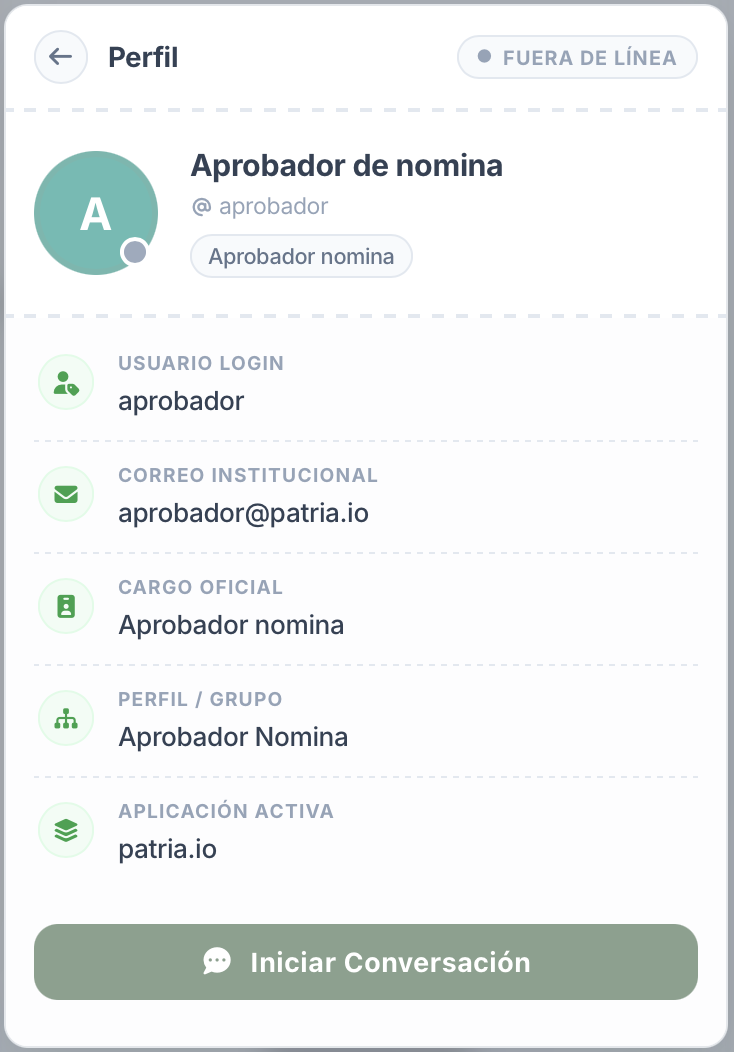
\includegraphics[width=0.7\textwidth]{anexos/22 chat.perfiles.png}}
\caption{Gestion de perfiles en el chat}
\label{fig:chat-perfiles}
\end{figure}

\notacientifica{Los perfiles de usuario permiten identificar rapidamente al emisor de cada mensaje.}

\subsection{Filtro de Contenido}

El sistema implementa sanitizacion proactiva de mensajes:

\begin{caja}{Medidas de Seguridad}
\begin{itemize}
\item \textbf{Prevencion de XSS}: Elimina codigo potencialmente malicioso
\item \textbf{Normalizacion de enlaces}: Valida URLs externas
\item \textbf{Detencion de comandos}: Previene la ejecucion de comandos inyectados
\item \textbf{Logging de seguridad}: Registra intentos de inyeccion
\end{itemize}
\end{caja}

\notacientifica{La sanitizacion proactiva protege tanto al usuario como al sistema de posibles ataques a traves del chat.}

\subsection{Historial y Auditoria}

El historial de chat proporciona un registro completo para auditorias:

\begin{caja}{Capacidades de Auditoria}
\begin{itemize}
\item \textbf{Registro completo}: Cada mensaje se almacena con todos los metadatos
\item \textbf{Busqueda avanzada}: Filtrar por usuario, fecha, contenido
\item \textbf{Exportacion}: Generar reportes de conversaciones
\item \textbf{Trazabilidad}: Cada mensaje puede rastrearse hasta su origen
\end{itemize}
\end{caja}

\notacientifica{Estas capacidades hacen del chat una herramienta valiosa para auditorias de seguridad y cumplimiento normativo.}
